\documentclass{article}
\usepackage[utf8]{vietnam}
\usepackage[12pt]{extsizes}
\usepackage{amsmath,amsfonts,amsthm}
\usepackage{mathrsfs}
\usepackage{enumitem}
\usepackage{geometry}
\usepackage{mathtools}
\usepackage{booktabs}
\usepackage{pgfplots}
\usepackage{amssymb}
\usepackage{array}
\usepackage{multirow}
\usepackage{tabularx}
\usepackage{hyperref}
 \geometry{
 a4paper,
 total={170mm,257mm},
 left=20mm,
 top=20mm,
 }
 \usepackage{graphicx}
 \usepackage{titling}
 \usepackage{listings}
 \title{Thiết kế bộ lọc IIR
}
\author{}
\date{Ngày 23/4/2025}
 \usepackage{fancyhdr}
\fancypagestyle{plain}{%  the preset of fancyhdr 
    \fancyhf{} % clear all header and footer fields
    \fancyfoot[L]{\thedate}
    \fancyhead[L]{}
    \fancyhead[R]{\theauthor}
}
\makeatletter\def\@maketitle{%
\newpage
\null
\vskip 1em%
\begin{center}%
\let \footnote \thanks
  {\LARGE \@title \par}%
  \vskip 1em%
  %{\large \@date}%
\end{center}%
\par
\vskip 1em}
\makeatother
\begin{document}
\maketitle
\section{Các bước thiết kế bộ lọc digital IIR}
\begin{enumerate}
  \item "Wrapping frequency", tức là phải chuyển tần số digital $\omega$ về tần số analog $\Omega$.
  \item Thiết kế bộ lọc analog theo các giá trị $\Omega$ tìm được ở bước trên.
  \begin{enumerate}
    \item Thiết kế bộ lọc lowpass prototype analog với $\Omega_{c}=1$ (c là cutoff frequency).
    \item Sử dụng "frequency transformation method" để chuyển để bộ lọc lowpass prototype về bộ lọc analog mong muốn.
    \item Cuối cùng, ta sẽ thu được một hàm $H(s)$ của bộ lọc mong muốn.
  \end{enumerate}
  \item Sử dụng các phép biến đổi như là "impulse invariance" hay biến đổi xung bậc thang hoặc thông dụng nhất là "bilinear transform" (biến đổi song tuyến tính) để chuyển hàm $H(s)\to H(z)$ tương ứng.
\end{enumerate}
\section{Thiết kế bộ lọc analog}
\subsection{Khái niệm và các họ mạch lọc LP, HP, BP và BS}
\begin{figure}[h]
  \begin{center}
  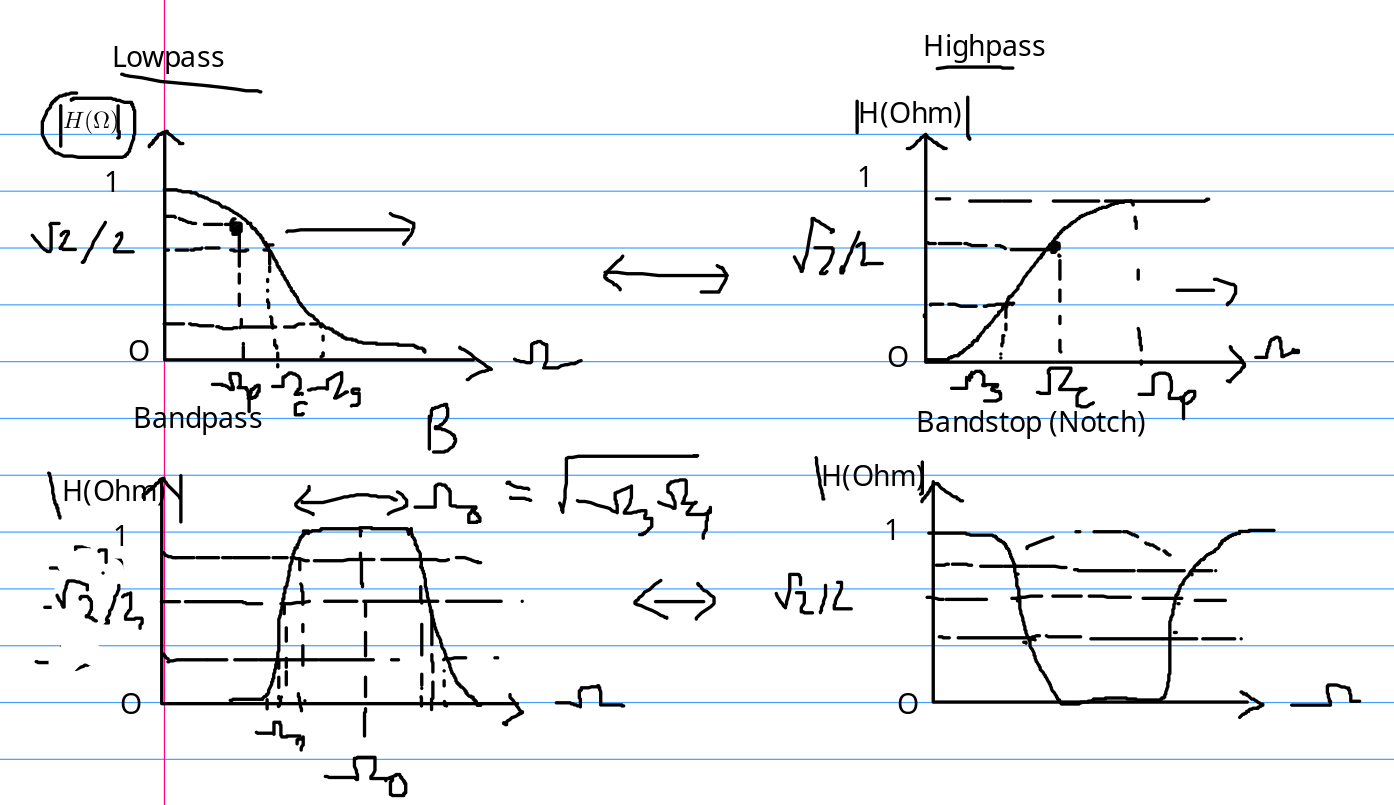
\includegraphics[width=16cm]{iir.png}
  \end{center}
  \end{figure} 
\subsection{Các loại mạch lọc}
\subsubsection{Mạch lọc Butterworth}
\begin{enumerate}
\item Khái niệm mạch lọc Butterworth: mạch lọc Butterworth là một mạch lọc không có gợn sóng và phẳng trên toàn bộ dải tần.
\item Đáp ứng biên độ của các họ mạch lọc Butterworth:
  \begin{enumerate}
    \item Bộ lọc LP: $$H(\Omega)=\frac{1}{\sqrt{1+\left(\frac{\Omega}{\Omega_{c}}\right)^{2n}}}$$
    \item Bộ lọc HP: $$H(\Omega)=\frac{1}{\sqrt{1+\left(\frac{\Omega_{c}}{\Omega}\right)^{2n}}}$$
    \item Bộ lọc BP: $$H(\Omega)=\frac{1}{\sqrt{1+\left(\frac{\Omega-\Omega_{0}}{\Omega_{c}}\right)^{2n}}}$$
    \item Bộ lọc BS: $$H(\Omega)=\frac{1}{\sqrt{1+\left(\frac{\Omega_{c}}{\Omega-\Omega_{0}}\right)^{2n}}}$$
  \end{enumerate}
  \item Thiết kế bộ lọc LP Butterworth prototype (tức là $\Omega_{c}=1$)
    \begin{enumerate}
      \item Biến đổi $|H(\Omega)|$ như sau:
      \begin{equation*}
        \begin{split}
          |H(\Omega)|^2=\frac{1}{1+\left(\Omega\right)^{2n}}=\frac{1}{1+\left(\frac{s}{j}\right)^{2n}}=H(s)H(-s)
        \end{split}
      \end{equation*}
      Để tìm các điểm cực $s$, ta phải giải phương trình $$\left(\frac{s}{j}\right)^{2n}=-1 \Leftrightarrow s_{k}=e^{\frac{j\pi}{2n}(2k+n-1)}$$
      \item Chọn các nghiệm cực $s_{k}$ để thỏa mãn hệ thống nhân quả và ổn định, tức là chọn sao cho $\Re(s)<0$.
      \item Viết lại phương trình hệ thống:$$H(s)=\frac{1}{(s-s_{1})(s-s_{2})...}=\frac{1}{B_{N}(s)}$$
      Mẫu số thu được gọi là đa thức Butterworth với bậc $N$.
    \end{enumerate}
    \item Thiết kế các họ bộ lọc khác từ bộ lọc LP Butterworth prototype:
    \begin{enumerate}
      \item Bộ lọc LP có $\Omega_{c}$ bất kì: $$s\to \frac{s}{\Omega_{c}}$$
      \item Bộ lọc HP có $\Omega_{c}$ bất kì: $$s\to \frac{\Omega_{c}}{s}$$
      \item Bộ lọc BP có $\Omega_{0}$ (tần trung bình hình học) và $B$ (bandpass) bất kì: $$s\to \frac{s^2+\Omega_{0}^2}{Bs}$$
      \item Bộ lọc BS có $\Omega_{0}$ (tần trung bình hình học) và $B$ (bandstop) bất kì: $$s\to \frac{Bs}{s^2+\Omega_{0}^2}$$
    \end{enumerate}
\end{enumerate}
\subsubsection{Mạch lọc Chebyshev}
\begin{enumerate}
  \item Khái niệm mạch lọc Chebyshev: là loại mạch lọc có gợn sóng trên 1 dải (passband hoặc stopband), ưu điểm so với mạch lọc Butterworth là transtion band, ở đây ta chỉ quan tâm đến
  Chebyshev type 1 (gợn sóng ở dải thông).
  \item Đáp ứng biên độ của các họ mạch lọc Chebyshev:
  \begin{enumerate}
    \item Bộ lọc LP: (ở đây sẽ dùng $|H(\Omega)|^2$ thay cho $|H(\Omega)|$ cho thuận quy ước các đại lượng khớp với slide cô Thịnh):
    $$|H(\Omega)|^{2}=\frac{\alpha}{1+\epsilon^2T_{N}^2\left(\frac{\Omega}{\Omega_{c}}\right)}$$
    \item Bộ lọc HP:
    $$|H(\Omega)|^{2}=\frac{\alpha}{1+\epsilon^2T_{N}^2\left(\frac{\Omega_{c}}{\Omega}\right)}$$
    \item Bộ lọc BP và BS không xét ở đây do được thiết kế gián tiếp thông qua bộ lọc LP prototype.
  \end{enumerate}
  \item Thiết kế bộ lọc LP Chebyshev prototype:
    \begin{enumerate}
      \item Tìm bậc $N$ của bộ lọc (bước này không dễ lắm và đôi lúc cũng hơi không chặt chẽ cho lắm), có nhiều cách để tìm bậc $N$, trong đó có cách dùng hàm $\cosh()$ (cân nhắc), nhưng mà nếu theo anh thì làm theo cách cô Thịnh, tức là nhìn đồ thị và đoán là ok.
      \item Tìm $\epsilon^2$, $\alpha$, cố gắng để xây dựng được hàm $|H(\Omega)|^2$, sau đó giải và tìm các cực $s_{k}$ như bước $3$ của mục thiết kế bộ lọc LP prototype Butterworth.
      \item Xây dựng hàm $H(s)$ như mục $3(c)$ phần Butterworth ở trên, nhưng lưu ý tử số có thể khác $1$ và phải điều chỉnh giá trị tử số thỏa mãn $|H(0)|=1$.
      \item Thiết kế các họ bộ lọc từ bộ lọc LP Chebyshev prototype: chuyển như ở trên.
    \end{enumerate}
\end{enumerate}
\subsection{Bài tập áp dụng}
\subsubsection{Một bộ lọc thông thấp có đáp ứng biên độ không quá $3dB$ trong khoảng tần số
$0-5kHz$. Độ suy hao trên $23dB$ với tần số trên $10kHz$. Xác định bậc của bộ lọc
Butterworth cần thiết kế. Nếu sử dụng Chebychev với độ gợn sóng $2.5dB$ thì bậc
bằng bao nhiêu?}
\begin{itemize}
  \item Thiết kế bộ lọc Butterworth:
  \begin{equation*}
    \begin{cases}
      0<|\Omega|<10^4\pi \:(rad/s)\quad(A>-3dB) \\ 
       |\Omega|>2.10^4\pi \:(rad/s)\quad(A<-23dB)\\
    \end{cases}
  \end{equation*}
  Từ phương trình của hàm đáp ứng biên độ Butterworth, ta có:
  $$A=20\log_{10}\left|H(\Omega)\right|=10\log_{10}|H(\Omega)|^2=10\log_{10}\frac{1}{1+\left(\frac{\Omega}{\Omega_{c}}\right)^{2n}}=-10\log_{10}\left[1+\left(\frac{\Omega}{\Omega_{c}}\right)^{2n}\right]$$
  Ta đã có từ dữ liệu của đề bài, dễ thấy $\Omega_{p}=\Omega_{c}=10^4\pi\:(rad/s)$ và $\Omega_{s}=2.10^4\pi\:(rad/s)$, ta sẽ tìm được bậc $N$ từ phương trình sau:
  $$A_{s}=-10\log_{10}\left[1+\left(\frac{\Omega_{s}}{\Omega_{c}}\right)^{2n}\right]$$
  Bấm máy ra $N=3.81$ thì ta lấy bậc của bộ lọc Butterworth là $N=4$.
  \item Thiết kế bộ lọc Chebyshev: nhìn đồ thị xác định được $N=3$ với gợn sóng $r=2.5dB$, làm tương tự như trên.
\end{itemize}
\section{Thiết kế bộ lọc Digital}
\subsection{Biến đổi theo đáp ứng xung}
Chỉ cần nhớ các công thức sau là sống:
\begin{equation*}
  \begin{split}
  \Omega&=\frac{\omega}{T_{s}}=\omega.f_{s}\\
  \omega&=\frac{2\pi f}{f_{{s}}}
  \end{split}
\end{equation*}
Biến đổi theo đáp ứng xung, tức là biến đổi từ hàm $H(s)$ về $H(z)$ như sau:
$$H(s)=\sum\frac{c_{i}}{s-\lambda}\to H(z)=\sum\frac{c_{i}Tz}{z-e^{\lambda T}}$$
\subsection{Biến đổi theo đáp ứng bậc thang}
Phần biến đổi tần số tương tự như đáp ứng xung, nhưng phần biến đổi $H(s)\to H(z)$ thì khác:
$$H(s)=\sum\frac{c_{i}}{s-p_{k}}\to H(z)=\sum\frac{1}{p_{k}}\left(\frac{e^{p_{k}T_{s}}-1}{z-e^{p_{k}T_{s}}}\right)$$
\subsection{Biến đổi theo phương pháp song tuyến tính}
Lưu ý lúc này phần biến đổi tần số sẽ khác:
$$\Omega=\frac{2}{T_{s}}\tan{\left(\frac{\omega}{2}\right)}$$
$$s=\frac{2}{T_{s}}\frac{1-z^{-1}}{1+z^{-1}}$$
\end{document}